\documentclass[11pt,a4paper]{article}
\usepackage[T1]{fontenc}
\usepackage[margin=2.3cm]{geometry}
\usepackage{amsmath,amssymb}
\usepackage{graphicx}
\usepackage[dvipsnames]{xcolor}
\usepackage{enumitem}
\usepackage[colorlinks=true,linkcolor=blue,urlcolor=blue]{hyperref}
\setlength{\parskip}{0.6em}
\setlength{\parindent}{0pt}
\begin{document}

\begin{center}{\LARGE\bfseries opengasturbine}\\[0.4em]{\large Predict the thrust and efficiency of a gas turbine with the Brayton cycle, in three sessions.}\\[0.2em]\small PAN IIT OSS explainer \textbullet{} higher secondary to advanced undergrad (levels 4-6)\end{center}

\section*{Why this exists}
Every airliner and many power stations run on a machine that squeezes air, burns fuel in it and lets the hot gas push back. This explainer shows the mathematics behind that: an energy balance, the ideal Brayton cycle and a turbojet with real losses that you can build yourself.

\section*{The end goal}
The end goal is to predict the thrust and efficiency of a gas turbine with the Brayton cycle. The same ideas carry over to turbofans, turboprops and the gas turbines of power stations, which differ in how they use the gas that leaves the turbine.

\section*{How the three sessions build up}
\begin{enumerate}[nosep]
\item \textbf{Session 1: Four parts and one energy balance: how a gas turbine makes work} (Level 1: conceptual interactive model, 60 min).
\item \textbf{Session 2: Cycle temperatures, net work and the best pressure ratio} (Level 2: mathematical engineering model, 75 min).
\item \textbf{Session 3: A turbojet with real losses: thrust, fuel use and validation} (Level 3: simulation and validation, 90 min).
\end{enumerate}

\section{Session 1: Four parts and one energy balance: how a gas turbine makes work}

\subsection*{A. Real-world problem}
A jet engine or a power-station gas turbine burns fuel to make power. Only part of the fuel's heat becomes useful work, and the rest leaves in the hot exhaust. How much work can we get from a given amount of heat, and why does an engine with a higher pressure ratio waste less?

\subsection*{B. Concept and theory}
A gas turbine is a loop with four parts. The compressor squeezes the incoming air to a higher pressure, which costs work w\_c. The combustor burns fuel in that air and adds the heat q\_in. The turbine lets the hot gas expand and gives work w\_t, which is more than the compressor took. The exhaust carries the unused heat q\_out away. Following one kilogram of air around the cycle, the air returns to its starting state and stores no energy, so energy in equals energy out: w\_net = q\_in - q\_out. The thermal efficiency is the useful work per unit of heat paid for, eta = w\_net / q\_in. For the ideal cycle (the Brayton cycle) the efficiency depends only on the pressure ratio r = p2 / p1: eta = 1 - 1 / r\textasciicircum{}K, with K = (gamma - 1) / gamma = 0.2857 for air. A higher r gives a higher eta, but the gain per unit of r gets smaller, and eta stays below 1 because some heat must always be rejected (the second law).

\begin{itemize}[nosep]
\item r: pressure ratio of the compressor, p2 / p1 (no unit)
\item gamma: ratio of specific heats of air (no unit (1.4))
\item K: (gamma - 1) / gamma (no unit (0.2857))
\item q\_in: heat added in the combustor per kg of air (kJ/kg)
\item w\_net: net work per kg of air (turbine work minus compressor work) (kJ/kg)
\item q\_out: heat rejected in the exhaust per kg of air (kJ/kg)
\item eta: thermal efficiency, w\_net / q\_in (no unit)
\end{itemize}

\[ w_{\mathrm{net}} = q_{\mathrm{in}} - q_{\mathrm{out}},\qquad \eta = \frac{w_{\mathrm{net}}}{q_{\mathrm{in}}} \]

\[ \eta = 1 - \frac{1}{r^{K}},\qquad K = \frac{\gamma - 1}{\gamma} \]

\subsection*{C. Visual explanation}
The first figure plots the ideal efficiency against the pressure ratio. The curve rises quickly at first and then flattens: going from r = 2 to r = 4 adds far more efficiency than going from r = 10 to r = 20. The red dot marks r = 10. The second figure shows the energy balance as three bars for 600 kJ of heat at r = 10: the heat in is split into the net work and the heat out.

\begin{figure}[h]\centering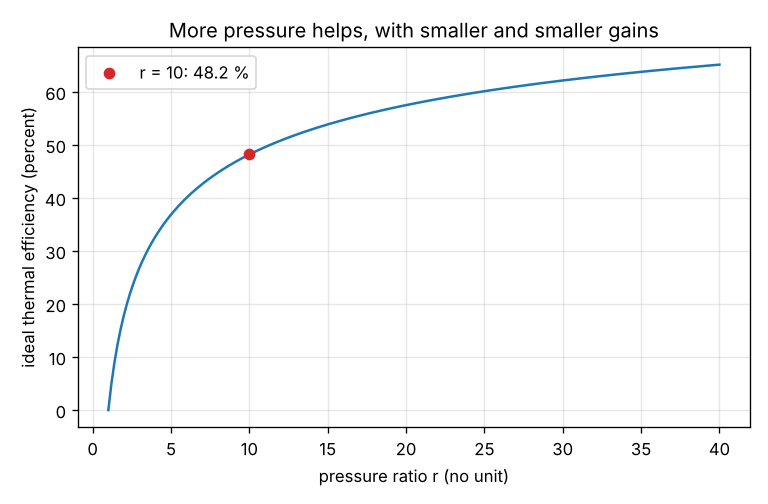
\includegraphics[width=0.78\textwidth]{figures/s01_efficiency_vs_ratio.png}\caption{Ideal efficiency against pressure ratio; the red dot is r = 10.}\end{figure}

\begin{figure}[h]\centering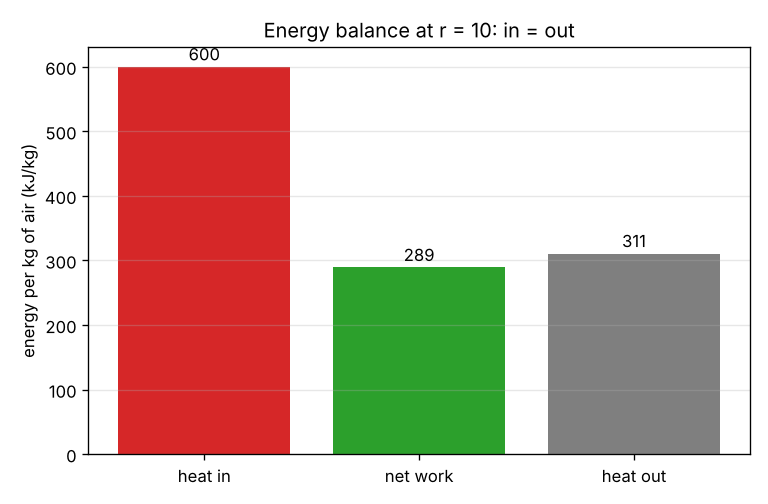
\includegraphics[width=0.78\textwidth]{figures/s01_energy_bars.png}\caption{Energy balance at r = 10 for 600 kJ/kg of heat: heat in equals net work plus heat out.}\end{figure}

\subsection*{E. Worked example}
\textbf{Problem.} Heat q\_in = 600 kJ per kg of air is added in an ideal gas turbine with pressure ratio r = 10. Find the efficiency, the net work and the heat rejected.

\begin{enumerate}[nosep]
\item K = (1.4 - 1) / 1.4 = 0.2857.
\item r\textasciicircum{}K = 10\textasciicircum{}0.2857 = 1.931.
\item eta = 1 - 1 / 1.931 = 0.482.
\item w\_net = eta x q\_in = 0.482 x 600 = 289 kJ/kg.
\item q\_out = q\_in - w\_net = 600 - 289 = 311 kJ/kg. Check: 289 + 311 = 600.
\end{enumerate}
\textbf{Answer.} Efficiency 0.482 (48.2 percent), net work 289 kJ/kg, heat rejected 311 kJ/kg.

\section{Session 2: Cycle temperatures, net work and the best pressure ratio}

\subsection*{A. Real-world problem}
A power-station turbine takes in 20 kg of air every second at 288 K. The metal of the turbine can survive gas at 1400 K. What are the temperatures at each point of the engine, how much power comes out, and which pressure ratio gives the most power? Is it also the pressure ratio with the best efficiency?

\subsection*{B. Concept and theory}
Number the states: 1 is the inlet, 2 the compressor exit, 3 the turbine inlet (the hottest point, set by the metal) and 4 the turbine exit. With no losses, compression and expansion follow T2 = T1 r\textasciicircum{}K and T4 = T3 / r\textasciicircum{}K. With a constant specific heat cp, every heat or work is cp times a temperature difference: w\_c = cp (T2 - T1), w\_t = cp (T3 - T4), q\_in = cp (T3 - T2) and q\_out = cp (T4 - T1). The net work is w\_net = w\_t - w\_c, and the efficiency w\_net / q\_in turns out to be 1 - 1 / r\textasciicircum{}K again, so the temperatures and Session 1 agree. For a fixed T1 and T3 the net work has a maximum: writing x = r\textasciicircum{}K and tau = T3 / T1, w\_net = cp T1 [tau (1 - 1/x) - (x - 1)], and setting the derivative with respect to x to zero gives x = sqrt(tau), that is r\_opt = (T3 / T1)\textasciicircum{}(1 / (2K)). Below r\_opt the gas leaves the turbine too hot (wasted potential); above it the compressor takes too much work. The efficiency, however, keeps rising with r, so the pressure ratio for the best work is not the one for the best efficiency.

\begin{itemize}[nosep]
\item T1, T2, T3, T4: temperatures at inlet, compressor exit, turbine inlet and turbine exit (K)
\item r: pressure ratio (no unit)
\item K: (gamma - 1) / gamma = 0.2857 (no unit)
\item cp: specific heat of air at constant pressure (kJ/(kg K), 1.005)
\item w\_c, w\_t, w\_net: compressor work, turbine work and net work per kg of air (kJ/kg)
\item q\_in: heat added per kg of air (kJ/kg)
\item mdot: air mass flow (kg/s)
\item P: net power, mdot x w\_net (kW (or MW))
\item r\_opt: pressure ratio for the largest net work (no unit)
\end{itemize}

\[ T_2 = T_1 r^{K},\qquad T_4 = \frac{T_3}{r^{K}} \]

\[ w_c = c_p (T_2 - T_1),\quad w_t = c_p (T_3 - T_4),\quad w_{\mathrm{net}} = w_t - w_c,\quad q_{\mathrm{in}} = c_p (T_3 - T_2) \]

\[ r_{\mathrm{opt}} = \left(\frac{T_3}{T_1}\right)^{\frac{1}{2K}} \]

\subsection*{C. Visual explanation}
The first figure plots the net work against the pressure ratio for three turbine inlet temperatures. Every curve rises, peaks and falls, and the peak (dot) moves to a higher pressure ratio and a higher work as T3 rises. The second figure shows how the two exit temperatures move: T2 climbs with r while T4 falls, and the two lines would meet T3 only at an impossible, very high pressure ratio.

\begin{figure}[h]\centering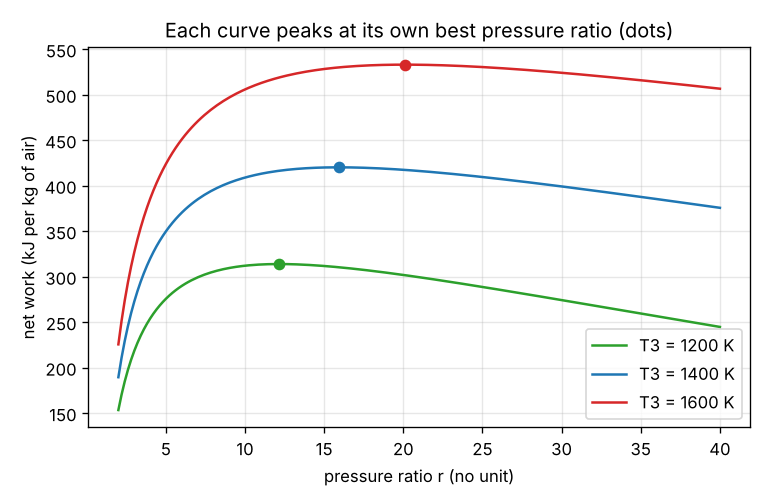
\includegraphics[width=0.78\textwidth]{figures/s02_work_vs_ratio.png}\caption{Net work against pressure ratio for three turbine inlet temperatures; the dots are the best ratios.}\end{figure}

\begin{figure}[h]\centering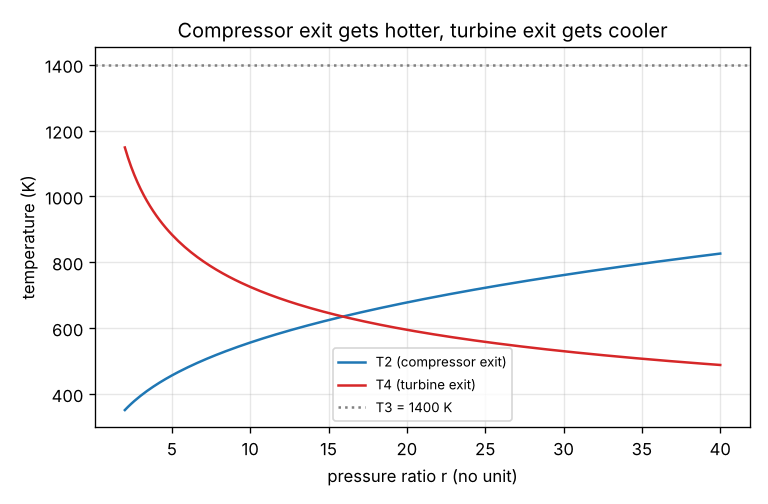
\includegraphics[width=0.78\textwidth]{figures/s02_temperatures_vs_ratio.png}\caption{Compressor exit and turbine exit temperature against pressure ratio at T3 = 1400 K.}\end{figure}

\subsection*{E. Worked example}
\textbf{Problem.} Air enters at T1 = 288 K, the pressure ratio is 10 and the turbine inlet temperature is T3 = 1400 K. The air flow is 20 kg/s. Find T2, T4, the works, the efficiency and the power.

\begin{enumerate}[nosep]
\item r\textasciicircum{}K = 10\textasciicircum{}0.2857 = 1.9307.
\item T2 = 288 x 1.9307 = 556.0 K and T4 = 1400 / 1.9307 = 725.1 K.
\item w\_c = 1.005 x (556.0 - 288) = 269.4 kJ/kg and w\_t = 1.005 x (1400 - 725.1) = 678.2 kJ/kg.
\item w\_net = 678.2 - 269.4 = 408.9 kJ/kg, and q\_in = 1.005 x (1400 - 556.0) = 848.2 kJ/kg.
\item eta = 408.9 / 848.2 = 0.4821, the same as 1 - 1 / r\textasciicircum{}K = 0.4821.
\item Power = 20 x 408.9 = 8177 kW = 8.18 MW.
\end{enumerate}
\textbf{Answer.} T2 = 556.0 K, T4 = 725.1 K, w\_net = 408.9 kJ/kg, eta = 0.482, power 8.18 MW.

\section{Session 3: A turbojet with real losses: thrust, fuel use and validation}

\subsection*{A. Real-world problem}
A jet engine does not make shaft power. The turbine takes only enough work to drive the compressor, and the rest of the hot gas expands through a nozzle and leaves fast; the push on the engine is the thrust. How much thrust does one kilogram of air per second give, how much fuel does it need, and how do the losses in the compressor, turbine and nozzle change the answer? Can we trust a model that has only a few numbers?

\subsection*{B. Concept and theory}
A real compressor needs more work than an ideal one, so with an isentropic efficiency eta\_c the exit temperature is T2 = T1 [1 + (r\textasciicircum{}K - 1) / eta\_c]. The turbine only drives the compressor, so T4 = T3 - (T2 - T1). A real turbine gives less work for the same pressure drop; with efficiency eta\_t the pressure left after the turbine follows (p4 / p3)\textasciicircum{}K = 1 - (T3 - T4) / (eta\_t T3), with p3 = r p1. The gas then expands in the nozzle from p4 down to the outside pressure p1: the ideal exit temperature is T5s = T4 (p1 / p4)\textasciicircum{}K and the nozzle efficiency eta\_n gives the temperature drop eta\_n (T4 - T5s), which becomes speed, v\_e = sqrt(2 cp eta\_n (T4 - T5s)). On a test stand the air enters at rest, so the thrust per kg/s of air is v\_e. The heat added is q\_in = cp (T3 - T2), and the fuel per kg of air is q\_in / (eta\_b LHV) with a lower heating value LHV = 43 MJ/kg and a combustor efficiency eta\_b = 0.98. The TSFC is the fuel flow per newton of thrust. To validate, two things must hold: with no losses the jet kinetic energy v\_e\textasciicircum{}2 / 2 equals the ideal net work of Session 2, and for any losses the heat added equals the enthalpy gain of the exhaust plus the jet kinetic energy.

\begin{itemize}[nosep]
\item eta\_c, eta\_t, eta\_n: isentropic efficiencies of compressor, turbine and nozzle (no unit)
\item T1 ... T5: temperatures at inlet, compressor exit, turbine inlet, turbine exit, nozzle exit (K)
\item p4 / p1: pressure ratio available to the nozzle (no unit)
\item v\_e: jet exit speed, equal to the specific thrust on a test stand (m/s = N s/kg)
\item cp: specific heat of air (J/(kg K), 1005)
\item LHV: lower heating value of the fuel (J/kg, 43e6)
\item eta\_b: combustor efficiency (no unit, 0.98)
\item fuel/air: fuel mass per kg of air, q\_in / (eta\_b LHV) (kg/kg)
\item TSFC: thrust specific fuel consumption (g/(kN s))
\end{itemize}

\[ T_2 = T_1\left[1 + \frac{r^{K}-1}{\eta_c}\right],\qquad T_4 = T_3 - (T_2 - T_1) \]

\[ \left(\frac{p_4}{p_3}\right)^{K} = 1 - \frac{T_3 - T_4}{\eta_t T_3},\qquad p_3 = r\,p_1 \]

\[ v_e = \sqrt{2 c_p\, \eta_n (T_4 - T_{5s})},\qquad T_{5s} = T_4\left(\frac{p_1}{p_4}\right)^{K} \]

\[ q_{\mathrm{in}} = c_p (T_3 - T_2) = c_p (T_5 - T_1) + \frac{v_e^2}{2} \]

\subsection*{C. Visual explanation}
The first figure plots the specific thrust against the pressure ratio for three turbine inlet temperatures. Each curve is nearly flat over a wide range of r and rises strongly with T3. The second figure plots the TSFC: it falls as the pressure ratio rises, which is why a high-pressure engine is more fuel-efficient, and every loss lifts the curve. Where a curve stops, the turbine cannot leave enough pressure for a jet.

\begin{figure}[h]\centering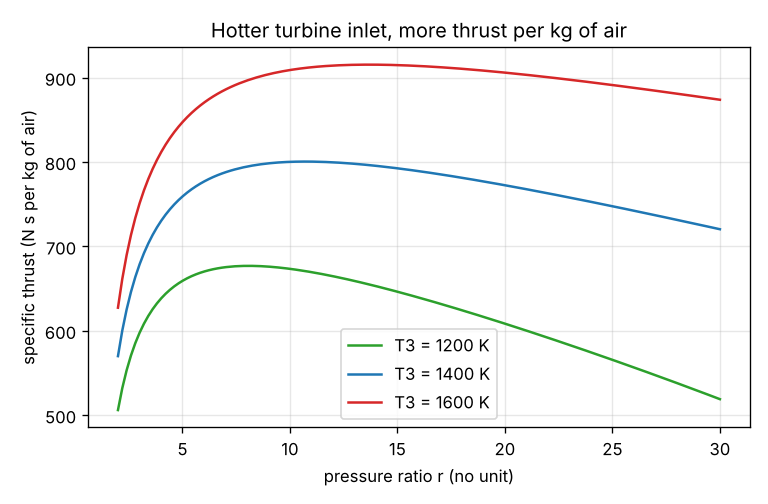
\includegraphics[width=0.78\textwidth]{figures/s03_thrust_vs_ratio.png}\caption{Specific thrust against pressure ratio for three turbine inlet temperatures.}\end{figure}

\begin{figure}[h]\centering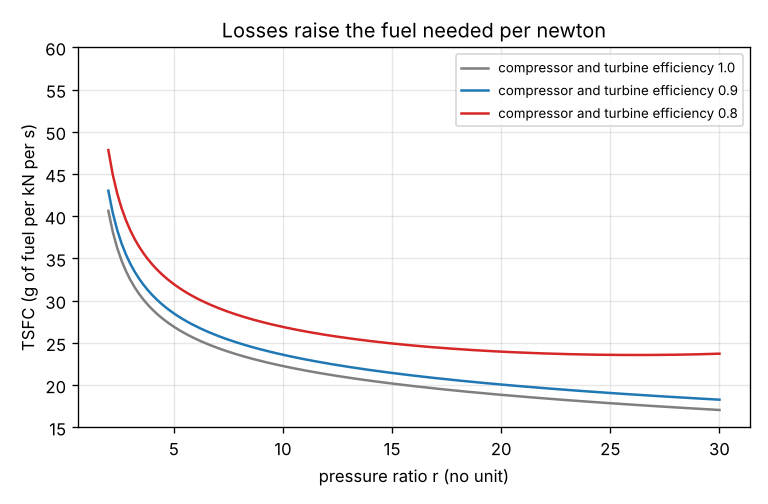
\includegraphics[width=0.78\textwidth]{figures/s03_tsfc_vs_ratio.png}\caption{Thrust specific fuel consumption against pressure ratio for three levels of component efficiency.}\end{figure}

\subsection*{E. Worked example}
\textbf{Problem.} A static turbojet takes in air at T1 = 288 K. The pressure ratio is 10, the turbine inlet temperature is T3 = 1400 K and the efficiencies are eta\_c = 0.85, eta\_t = 0.90 and eta\_n = 0.95. Find the specific thrust, the TSFC and, for 20 kg/s of air, the thrust and the fuel flow.

\begin{enumerate}[nosep]
\item T2 = 288 x [1 + (1.9307 - 1) / 0.85] = 603.3 K.
\item T4 = 1400 - (603.3 - 288) = 1084.7 K.
\item (p4 / p3)\textasciicircum{}K = 1 - 315.3 / (0.90 x 1400) = 0.7497, so p4 / p3 = 0.3649 and p4 / p1 = 3.65.
\item T5s = 1084.7 x (1 / 3.65)\textasciicircum{}0.2857 = 749.3 K, so the nozzle drop is 0.95 x (1084.7 - 749.3) = 318.6 K.
\item v\_e = sqrt(2 x 1005 x 318.6) = 800 m/s, which is the specific thrust: 800 N s/kg.
\item q\_in = 1005 x (1400 - 603.3) = 800.6 kJ/kg, so fuel/air = 800.6e3 / (43e6 x 0.98) = 0.0190 and TSFC = 0.0190 / 800 = 23.7 g/(kN s).
\item For 20 kg/s: thrust = 20 x 800 = 16.0 kN and fuel = 20 x 0.0190 = 0.38 kg/s.
\end{enumerate}
\textbf{Answer.} Specific thrust 800 N s/kg, TSFC 23.7 g/(kN s); for 20 kg/s of air: 16.0 kN of thrust and 0.38 kg/s of fuel.

\section*{Where to go next}
\begin{enumerate}[nosep]
\item \textbf{Flight speed and ram compression.} Add the flight Mach number to the turbojet: total temperature and pressure at the inlet, and thrust per kg of air equal to v\_e - v\_0.
\item \textbf{Pressure losses in the inlet, combustor and nozzle.} Add a total pressure ratio for each of the three parts and carry them through the cycle.
\item \textbf{Variable gas properties.} Use two sets of properties (cold air and hot combustion gas) in the same cycle code.
\item \textbf{Turbine cooling air.} Bleed a fraction of the compressor air past the combustor and mix it back at the turbine.
\item \textbf{The turbofan: bypass ratio and propulsive efficiency.} Add a bypass duct with its own fan and compute the thrust of the core and of the bypass stream.
\end{enumerate}

This is a simplified educational model. It is not a validated design tool and must not be used for real structures, electrical installations, vehicles, industrial processes or medical decisions.

\end{document}
